\section{Experiments}
\label{sec:experiments}

\textbf{Setup.} Development experiments use one clip, a climb onto a 0.84\,m box, at its five box heights (0.67 to 1.01\,m): five tasks. They train 4{,}096 worlds for 59 million samples with 320 evaluation worlds on the side, three seeds per setting. Samples count the steps of training worlds; evaluation worlds add 8\% of simulation that we do not count. The tracker that teaches the reference worlds is trained once, for 74 million samples, and shared by all settings. ``Success holds from $n$ samples'' means that the evaluation success, logged every 2.5 million samples, stays at or above the level from $n$ on. All-clip experiments use 8{,}192 training worlds and 1{,}680 evaluation worlds. Everything runs on one RTX PRO 6000 GPU.

\subsection{What each kind of world causes}
\label{sec:cause}

Table~\ref{tab:cause} isolates the kinds of worlds on the development tasks.

\emph{Goal worlds alone learn nothing.} With the Boolean, the survival term, and starts on clip frames up to the one before the goal, success is \causeGoal{} from every rung in every seed, including starts where the robot already stands on the box. A humanoid does not stay upright by chance for the second that separates it from the first reward.

\emph{A tracker solves the clip start and nothing else.} It succeeds in \causeTrackerClip{} of episodes from the first frame and \causeTrackerAway{} from displaced starts; it follows the clip where the clip is, not where the robot is.

\emph{Reference worlds give the motion to a policy that cannot see the clip.} Trained on reference worlds only, the policy reaches \causeRefClip{} from the clip start. It has learned which motion belongs to which state. From displaced starts it reaches \causeRefAway{}: more than the tracker, because its goal is relative to the robot, and far from solved.

\emph{Goal worlds turn the motion into the task.} With goal worlds for half of the worlds, success from displaced starts rises to \causeHybridAway{} while the clip start stays at \causeHybridClip{}.

\emph{The teacher is what lets the two kinds mix from the start.} \causeNoTeacher{}

So the causes are separable and ordered: reference worlds cause success on the clip, goal worlds cause success away from it, and the second needs the first. This is the structure the rule of Sec.~\ref{sec:rule} assumes.

\begin{table}[t]
\centering
\caption{What each kind of world causes: success on the development tasks after 59 million samples. Mean of three seeds, with their range; the tracker is one run.}
\label{tab:cause}
\begin{tabular}{@{}lcc@{}}
\toprule
Worlds that train the policy & Clip start & Displaced start \\
\midrule
Goal worlds only & 0.00 \,{\scriptsize(0.00--0.00)} & 0.00 \,{\scriptsize(0.00--0.00)} \\
Tracker (observes the clip) & 0.84 & 0.05 \\
\midrule
Reference worlds, tracking reward & 0.59 \,{\scriptsize(0.00--0.93)} & 0.29 \,{\scriptsize(0.00--0.45)} \\
Reference worlds, teacher & 0.92 \,{\scriptsize(0.91--0.93)} & 0.25 \,{\scriptsize(0.24--0.26)} \\
Both, tracking reward & 0.00 \,{\scriptsize(0.00--0.00)} & 0.00 \,{\scriptsize(0.00--0.00)} \\
Both, teacher & 0.98 \,{\scriptsize(0.96--0.99)} & 0.92 \,{\scriptsize(0.92--0.93)} \\
\bottomrule
\end{tabular}

\end{table}

\subsection{The share is a strong and one-sided lever}
\label{sec:share}

Fig.~\ref{fig:sweep} sweeps a fixed share of reference worlds. With a share of 0.10 the policy learns nothing in the budget: the goal worlds, which cannot yet be rewarded, outnumber the worlds that teach. With 0.25 and 0.50 it reaches both success levels. With 0.75 it is slow away from the clip, and with 1.00 it stays tied to the clip. A hand-set share therefore has a cliff on one side and a slope on the other, and a practitioner finds the safe region by a sweep of full training runs.

\begin{figure}[t]
\centering
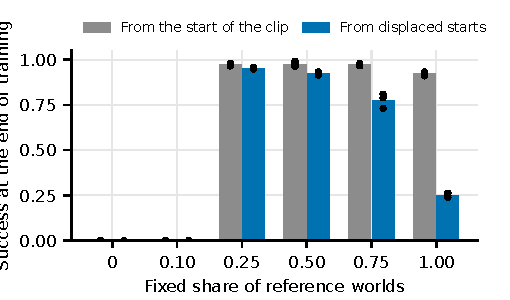
\includegraphics[width=\columnwidth]{figs/sweep_dev.pdf}
\caption{Success at the end of training for fixed shares of reference worlds. Bars are means of three seeds, dots the seeds.}
\label{fig:sweep}
\end{figure}

\subsection{Allocation by the evaluation against hand schedules}
\label{sec:schedules}

Table~\ref{tab:schedules} and Fig.~\ref{fig:schedules} compare ways to set the share. All use the same reference worlds, teacher, and goal worlds.

\emph{Hand schedules.} ``Two stages'' trains reference worlds alone for two thirds of the budget and then an even split, the proportions of~\cite{hil}. ``Tracking progress'' lowers the share from 1.0 to 0.5 in steps while fewer than 30\% of the reference episodes lose their clip, in the manner of~\cite{wang2026generalizing}. Both reach the clip-start level early, because they start with references only, and the displaced level late, because they hold goal worlds back by a clock or by a statistic of the wrong task.

\emph{The credit rule} reads the evaluation worlds every 100 iterations. \scheduleSentence{}

\emph{Trial learners.} The two learners that try shares 0.15 above and below the current one choose the reference-heavy share for the first \trialSamples{} million samples and then walk the share down to about 0.2 (Fig.~\ref{fig:schedules}, right). This is the direction the rule takes, measured by intervention rather than assumed. Its cost is as predicted: each learner has half of the worlds, and the pair needs \trialCost{} the samples of the rule.

\emph{Without the teacher} the picture changes (lower block of Table~\ref{tab:schedules}). \noTeacherSentence{}

\begin{table}[t]
\centering
\caption{Ways to set the share of reference worlds on the development tasks. Mean and range of the seeds: three with the teacher, two or three without. [$n/m$]: the $n$ of $m$ seeds that got there; ``never'': none within 59 million samples.}
\label{tab:schedules}
\setlength{\tabcolsep}{3pt}
\resizebox{\columnwidth}{!}{\begin{tabular}{@{}lcccc@{}}
\toprule
 & \multicolumn{2}{c}{Samples (M) until success holds} & \multicolumn{2}{c}{Success at 59\,M} \\
Share of reference worlds & clip $\geq$0.9 & displaced $\geq$0.8 & clip & displaced \\
\midrule
Goal worlds only & never & never & 0.00 \,{\scriptsize(0.00--0.00)} & 0.00 \,{\scriptsize(0.00--0.00)} \\
\midrule
\multicolumn{5}{@{}l}{\emph{Reference worlds taught by a tracker}} \\
Fixed share 0.10 & never & never & 0.00 \,{\scriptsize(0.00--0.00)} & 0.00 \,{\scriptsize(0.00--0.00)} \\
Fixed share 0.25 & 35 \,{\scriptsize(32--39)} & 38 \,{\scriptsize(34--42)} & 0.98 \,{\scriptsize(0.97--0.98)} & 0.95 \,{\scriptsize(0.95--0.96)} \\
Fixed share 0.50 & 26 \,{\scriptsize(25--27)} & 37 \,{\scriptsize(37--37)} & 0.98 \,{\scriptsize(0.96--0.99)} & 0.92 \,{\scriptsize(0.92--0.93)} \\
Fixed share 0.75 & 34 \,{\scriptsize(29--39)} & 57 \,{\scriptsize[1/3]} & 0.97 \,{\scriptsize(0.97--0.98)} & 0.78 \,{\scriptsize(0.73--0.81)} \\
Fixed share 1.00 & 50 \,{\scriptsize(47--57)} & never & 0.92 \,{\scriptsize(0.91--0.93)} & 0.25 \,{\scriptsize(0.24--0.26)} \\
Two stages~\cite{hil} & 44 \,{\scriptsize(42--47)} & 53 \,{\scriptsize(52--57)} & 0.98 \,{\scriptsize(0.97--0.98)} & 0.85 \,{\scriptsize(0.84--0.87)} \\
Tracking progress~\cite{wang2026generalizing} & 31 \,{\scriptsize(29--32)} & 43 \,{\scriptsize(42--47)} & 0.98 \,{\scriptsize(0.97--0.99)} & 0.91 \,{\scriptsize(0.90--0.91)} \\
Two trial learners & 51 \,{\scriptsize(47--54)} & 45 \,{\scriptsize(42--49)} & 0.95 \,{\scriptsize(0.95--0.96)} & 0.88 \,{\scriptsize(0.86--0.89)} \\
Credit rule without gates & 25 \,{\scriptsize(22--27)} & 27 \,{\scriptsize(27--27)} & 0.98 \,{\scriptsize(0.97--0.99)} & 0.95 \,{\scriptsize(0.94--0.96)} \\
Credit rule (ours) & 22 \,{\scriptsize(17--27)} & 22 \,{\scriptsize(22--22)} & 0.98 \,{\scriptsize(0.96--0.99)} & 0.95 \,{\scriptsize(0.94--0.97)} \\
\midrule
\multicolumn{5}{@{}l}{\emph{Reference worlds with the tracking reward only}} \\
Fixed share 0.50 & never & never & 0.00 \,{\scriptsize(0.00--0.00)} & 0.00 \,{\scriptsize(0.00--0.00)} \\
Fixed share 1.00 & 54 \,{\scriptsize(52--57)} \,{\scriptsize[2/3]} & never & 0.59 \,{\scriptsize(0.00--0.93)} & 0.29 \,{\scriptsize(0.00--0.45)} \\
Two stages~\cite{hil} & 47 \,{\scriptsize[1/2]} & 57 \,{\scriptsize[1/2]} & 0.49 \,{\scriptsize(0.00--0.98)} & 0.41 \,{\scriptsize(0.00--0.82)} \\
Tracking progress~\cite{wang2026generalizing} & never & never & 0.46 \,{\scriptsize(0.00--0.91)} & 0.24 \,{\scriptsize(0.00--0.47)} \\
Credit rule without gates & never & never & 0.00 \,{\scriptsize(0.00--0.00)} & 0.00 \,{\scriptsize(0.00--0.00)} \\
Credit rule & never & never & 0.00 \,{\scriptsize(0.00--0.00)} & 0.00 \,{\scriptsize(0.00--0.00)} \\
\bottomrule
\end{tabular}
}
\end{table}

\begin{figure*}[t]
\centering
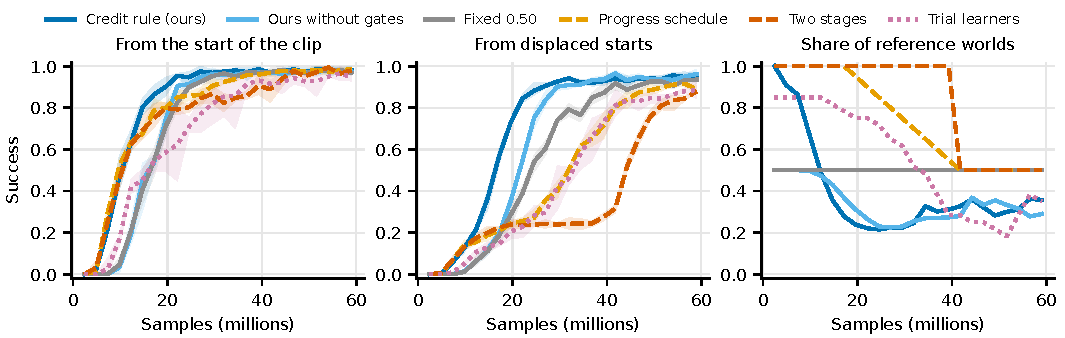
\includegraphics[width=\textwidth]{figs/schedules_dev.pdf}
\caption{Success from the clip start and from displaced starts during training, and the share of reference worlds that each method uses. Lines are means of three seeds, bands their range.}
\label{fig:schedules}
\end{figure*}

\subsection{Away from the clip}

Fig.~\ref{fig:displaced} moves the start further than training did. The policy was trained with displacements up to 0.5\,m and 0.5\,rad. It succeeds in \displacedHalf{} of episodes at that range, \displacedThreeQuarters{} at 0.75, and \displacedOne{} at 1.0; the tracker is at \displacedTrackerQuarter{} already at 0.25 and at \displacedTrackerOne{} at 1.0. Fig.~\ref{fig:teaser} shows one such episode.

\begin{figure}[t]
\centering
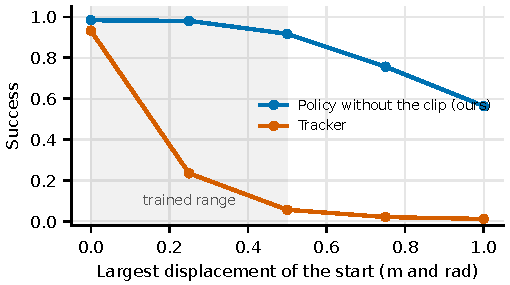
\includegraphics[width=\columnwidth]{figs/displaced.pdf}
\caption{Success from starts displaced by up to the amount on the horizontal axis, along both ground axes and in heading, over about a thousand episodes per point.}
\label{fig:displaced}
\end{figure}

\subsection{All clips, one policy}
\label{sec:all}

We train one tracker and then one policy on all \tasksall{} tasks, with 8{,}192 training worlds. The credit rule now also spreads the worlds of each kind over the tasks.

\emph{The tracker.} After \fullTrackerSamples{} million samples the tracker succeeds from the clip start in \fullTrackerClip{} of episodes averaged over the tasks, and in \fullTrackerAway{} from displaced starts. It solves \fullTrackerSolved{} of the \tasksall{} tasks at 0.5 or better. The tasks it does not solve are mostly the tallest boxes and three clips whose climbs it never completes; a second stage of training on the partly solved tasks gained 0.01 per 25 million samples and was stopped.

\emph{The policy.} Fig.~\ref{fig:full} shows the policy trained with the credit rule and this tracker as its teacher. \fullSentence{}

\emph{Past the teacher.} Fig.~\ref{fig:fulltasks} shows where. \fullTasksSentence{} The rule's gate gives these tasks few reference worlds, because the teacher cannot show them; what solves them is the Boolean in goal worlds, on a policy that has learned to climb elsewhere. A tracker cannot do this: it has no goal to be rewarded for.

\begin{figure}[t]
\centering
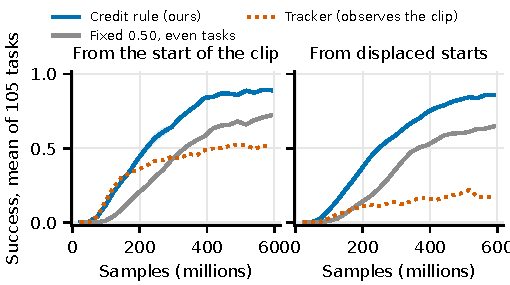
\includegraphics[width=\columnwidth]{figs/full_curves.pdf}
\caption{All \tasksall{} tasks, one policy. The policy does not observe a clip; the tracker that teaches it does. Credit rule: mean and range of \seedsAll{} seeds.}
\label{fig:full}
\end{figure}

\begin{figure*}[t]
\centering
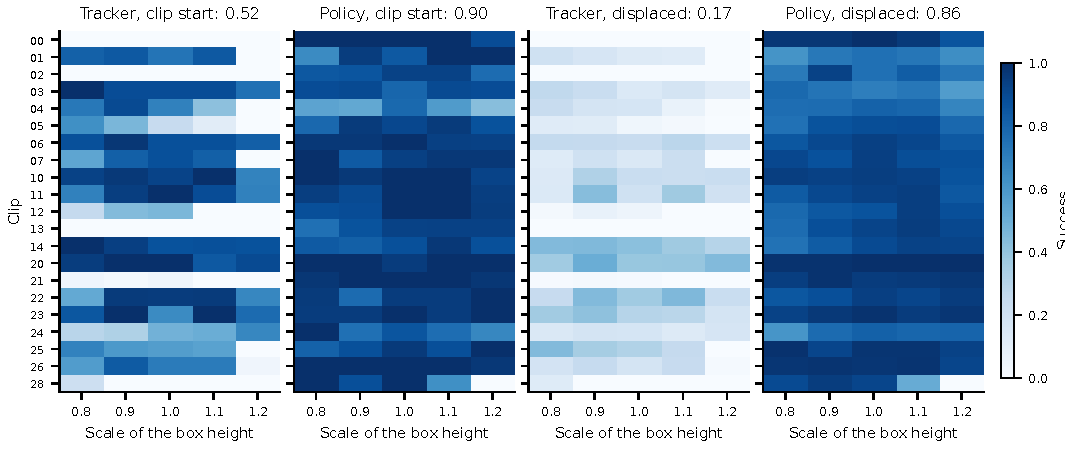
\includegraphics[width=\textwidth]{figs/full_tasks.pdf}
\caption{Success on every task at the end of training: a row per clip, a column per scale of the box height, and the mean over the tasks in each title. The policy is its first seed.}
\label{fig:fulltasks}
\end{figure*}

\subsection{Tasks that no world trained}

Does the policy climb boxes it never trained on? We repeat the run with tasks held out: no reference world and no goal world is ever placed on them, and the evaluation worlds still measure them (Table~\ref{tab:heldout}). \heldoutSentence{}

\begin{table}[t]
\centering
\caption{Tasks held out of training: no world of either kind is placed on them. Success averaged over the tasks.}
\label{tab:heldout}
\setlength{\tabcolsep}{4pt}
\begin{tabular}{@{}lccccc@{}}
\toprule
 & & \multicolumn{2}{c}{Tasks trained on} & \multicolumn{2}{c}{Tasks held out} \\
Held out of training & Tasks & clip & displaced & clip & displaced \\
\midrule
Two of five box heights & 42 & 0.87 & 0.80 & 0.90 & 0.81 \\
Five of 21 clips & 25 & 0.83 & 0.80 & 0.48 & 0.46 \\
\bottomrule
\end{tabular}

\end{table}

\subsection{Training time}

\timeSentence{}


\section{What Did Not Work}

We list what failed, because several of these are natural first choices. (i) A per-step penalty for tilt with termination on a fall rewards falling early, since every step survived costs reward; we replaced it with a survival term, and goal worlds alone still learned nothing. (ii) Starting worlds on the stretch of the clip where the evaluation ladder shows episodes being lost, a reverse curriculum read from the ladder, was worse than uniform starts for the tracker: it learned the last stretch first and never the ones before (0.00 against \lossStarts{} from the clip start at 25 million samples). (iii) With the reduced collision geometry of the robot, the tracker lost the clip in half of its episodes, at the climb, against one in twenty with the full geometry.

\section{Limitations}
\label{sec:limits}

All results are in simulation, with a state-based policy that observes quantities a robot must estimate, without domain randomisation; we have not run the policy on hardware. The rule needs the teacher: with the tracking reward alone it learns nothing, because it places a few goal worlds from the first iteration. The rule encodes two causal relations that we measured on these tasks; a task family in which goal worlds teach without references, or references mislead, needs them measured again, which the trial learners do at twice the cost. Success is defined by the pose of the pelvis, so the policy is not asked to move like the clip, and we did not measure how closely it does. The displaced starts are within a metre of the clip start and always in front of the box. We report three seeds for the development experiments, \seedsAll{} for the policy on all clips, and one for each other experiment on all clips. Without the teacher, the tracking reward taught the climb in some runs and not in others, and we do not know what separates them.

\section{Conclusion}

Clips can give a goal-driven policy what a Boolean reward cannot, but only through worlds that are there for a reason. We measured the reasons: reference worlds cause the motion, goal worlds cause its use away from the clip, and the second waits for the first. Stated as a rule that reads evaluation worlds, they replace the hand schedules of hybrid imitation, reach the same success in about half the samples with no setting to tune, and carry one policy past its teacher, onto tasks the teacher never solved. What the rule cannot do is start without a teacher. Removing that dependence and running the policy on the robot are the next steps.
